\documentclass[10pt,a4paper]{article}

% Encoding and fonts
\usepackage[utf8]{inputenc}
\usepackage[T1]{fontenc}
\usepackage{lmodern}

% Math and symbols
\usepackage{amsmath, amssymb, amsfonts}

% Graphics and figures
\usepackage{graphicx}
\usepackage{caption}
\usepackage{subcaption}
\usepackage{tikz}
\usetikzlibrary{arrows.meta,positioning,fit,shapes.multipart,calc,fit}

% Better referencing
\usepackage{hyperref}
\usepackage{cleveref}

% Bibliography
\usepackage[numbers]{natbib}
\bibliographystyle{apalike}

% Formatting
\usepackage{setspace}
\onehalfspacing
\usepackage{geometry}
\geometry{margin=2.5cm}

% Title info
\title{Semester Project Report \\ \large Neural Networks (AI)}
\author{
  Team Members: David van Wuijkhuijse (s5592968), \\Marcus Harald Olof Persson (s5343798), \\Richard Frank Harnisch (s5238366) \\
  University of Groningen
}
\date{\today}

\begin{document}

\maketitle

\begin{abstract}
  \noindent
  We implemented a feed-forward convolutional neural network from the group up including loss, activations, optimizer, and LR scheduler. We trained and evaluated the model on the German Traffic Sign Recognition Benchmark (GTSRB) dataset with 38 classes. Our model achieved a test accuracy of xx\%.
\end{abstract}

\tableofcontents
\newpage

\section{Introduction}
With this project, we implemented the 1998 CNN introduced by \citeauthor{LeCun-1998} (\citeyear{LeCun-1998}) using our own architecture coded from scratch in Python. We then would deploy this CNN on the German Traffic Sign Recognition Benchmark (GTSRB), consisting of 51,389 images and 43 classes. The dataset contains images with varying sizes and conditions, requiring different kinds of preprocessing steps, described in our pipeline.

Our main goal of this project is to create the core components of a CNN -- think convolution and pooling -- from scratch, only using lower-level libraries (e.g. Numpy, Pillow) in Python. The motivation behind this decision was to gain further insights into how neural networks work, by understanding and implementing the math behind the components of the CNN. We evaluated model performance using the accuracy metric and confusion matrices. We considered a model having a higher accuracy metric than 50\% (random guessing baseline) to be successful. 

\section{Data}
The German Traffic Sign Recognition Benchmark (GTSRB) dataset consists of 51,839 images of traffic signs on German roads, categorized into 43 different classes. The images are taken from dashcam footage of cars driving on the road and thus past the signs. This means that each sign is captured multiple times as the car passes the sign. This lessens the need for data augmentation as each sign is already represented multiple times. Signs are captured in a range of different lighting and weather conditions, as well as from different angles and distances.
\begin{figure}[h]
  \centering
  \includegraphics[width=0.3\textwidth]{images/00000_00000_00000.png}
  \includegraphics[width=0.3\textwidth]{images/00000_00000_00015.png}
  \includegraphics[width=0.3\textwidth]{images/00000_00000_00029.png}
  \caption{The same sign from different distances (and thus sizes) and slightly different angles.}
  \label{fig:augmentation}
\end{figure}
\begin{figure}[h]
  \centering
  \includegraphics[width=0.3\textwidth]{images/00001_00001_00005.png}
  \includegraphics[width=0.3\textwidth]{images/00001_00006_00014.png}
  \includegraphics[width=0.3\textwidth]{images/00001_00012_00014.png}
  \caption{Three different signs of the same type exhibiting variation in lighting conditions and angles. For more examples of different types of variation, see Figure \ref{fig:random-samples} in Appendix \ref{appendix:materials}.}
  \label{fig:variation}
\end{figure}

The dataset is provided by Stallkamp et al. (2012) \cite{Stallkamp-IJCNN-2011} \cite{Stallkamp2012} from the Institute for Neuroinformatics at the University of Bochum in Germany. By default, the dataset is split into a training set and a testing set. This was originally for a competition at the International Joint Conference on Neural Networks in 2011. Considering we are (considerably) past the deadline for submission, we have chosen to merge the training and testing sets at download time and then create our own split. This allows us to modify the split ratio as we like.

The images themselves are presented as PPM files with varying resolution and aspect ratio depending on the distance and angle of the sign to the camera. The aspect ratio is mostly close to 1:1. For more detailed analysis of the images sizes see Table \ref{tab:image-stats} and Figure \ref{fig:image-dimensions}. There are three color channels (RGB) and the pixel values are in the range of 0-255. See Figure \ref{color-histogram} for the distribution of pixel values. The labels for the images are provided in one master file \texttt{labels.csv} for the entire dataset. Each line contains the filename, class ID, and bounding box coordinates for the sign in the image.

\begin{table}
  \centering
  \begin{tabular}{lrrr}
    Statistic                & Width (px) & Height (px) & Aspect Ratio (W/H) \\
    \hline
    Mean                     & 50.76      & 50.34       & 1.0056             \\
    Std                      & 24.50      & 23.26       & 0.0734             \\
    Min                      & 25         & 25          & 0.3681             \\
    25th Percentile          & 34         & 35          & 0.9706             \\
    50th Percentile (Median) & 43         & 43          & 1.0000             \\
    75th Percentile          & 58         & 58          & 1.0385             \\
    Max                      & 266        & 232         & 1.4375             \\
    \hline
  \end{tabular}
  \caption{Descriptive statistics of image dimensions and aspect ratios in the GTSRB dataset.}
  \label{tab:image-stats}
\end{table}

\begin{figure}
  \centering
  \includegraphics[width=0.45\textwidth]{images/histogram_dimensions.png}
  \includegraphics[width=0.45\textwidth]{images/histogram_ratio.png}
  \caption{Distribution of image dimensions and aspect ratios in the GTSRB dataset. Most images are around 30-70 pixels in both dimensions, with a long tail towards larger sizes.}
  \label{fig:image-dimensions}
\end{figure}

\begin{figure}
  \centering
  \includegraphics[width=0.9\textwidth]{images/histogram_color.png}
  \caption{Histogram of pixel values across all images and color channels in the GTSRB dataset. The graph is cut off at frequency=50, but the frequency of flat white is very high due to the reflective nature of signs as well as the common use of the color white, causing (parts of) signs to max out the camera's sensor.}
  \label{color-histogram}
\end{figure}

\begin{figure}
  \centering
  \includegraphics[width=0.9\textwidth]{images/class_distribution.png}
  \caption{Class distribution of the GTSRB dataset. The dataset is imbalanced, with the smallest class having 270 images and the largest 3000. The mean is 1206 images per class.}
  \label{class-distribution}
\end{figure}

We load the data as a numpy array of shape (H, W, C) for each image, where H is height, W is width, and C is the color channel (so three). The labels are loaded as integers corresponding to the class IDs. Before feeding the images to the model, we normalize the pixel values to the range [0, 1] by dividing by 255.

\begin{itemize}
  \item Source of dataset
  \item Size and type (tabular, images, time series…)
  \item Key characteristics (with plots or descriptive stats)
  \item Any preprocessing or cleaning
\end{itemize}

Data is downloaded and cleaned automatically using the \texttt{dataio/gtsrb\_download.py} script. This script downloads the zipped dataset (three files: training dataset including labels, test dataset, test dataset labels), merges all images into one folder, and creates one master CSV file with all labels. It then deleted the zip files unless a parameter is set to keep them, as well as cleans the folder structure to remove unnecessary files (dataset text info files) and now empty folders. The data is freely hosted online by the University of Copenhagen Electronic Research Data Archive.

We implement a GTSRB dataset class in \texttt{dataio/gtsrb\_dataset.py}. This class handles loading the images and labels from disk, applying any specified transforms, and providing access to individual samples. This is meant as a minimal implementation of the PyTorch Dataset class. The dataset provides access to a length attribute (number of samples) and a getitem method to retrieve individual samples by index (returns a tuple of image and label). The dataset class also supports caching of images in memory for faster access during training, as well as multiple worker threads for parallel loading of data. These performance optimizations were implemented later in the project after initial tests showed slow training.

\section{Methods and Experiments}
\subsection{Pipeline Overview}
To begin, we preprocess the data. For this purpose, we have developed a suite of modular transform classes implemented in \texttt{transforms.py}. Each class implements a \texttt{\_\_call\_\_} method, allowing instances of these classes to be used as callable functions that apply specific transformations to input images. This design enables easy composition of multiple transformations into a single pipeline using the \texttt{ToCompose} class, which sequentially applies a list of transform instances to an image. On top of this, the following classes are implemented:
\begin{itemize}
  \item \texttt{ToResize}: Resizes images to a specified square size using bicubic interpolation. This is so the images can be fed into the model which requires a fixed input size.
  \item \texttt{ToCenterCrop}: Crops a square out of the center of an image to a specified pixel size.
  \item \texttt{ToGrayscale}: Converts RGB images to grayscale using the ITU-R
        601-2 luma transform using the formula
        \begin{equation}
          L = \frac{1}{1000}(299 R + 587 G + 114 B),
        \end{equation}
        where $R$, $G$, and $B$ are the red, green, and blue pixel values, respectively. This is implemented by the PIL library. We then convert back to RGB by duplicating the grayscale channel three times, as the network expects three channels.
  \item \texttt{ToTensor}: Converts images from numpy arrays to PyTorch tensors and permutes the dimensions from (H, W, C) to (C, H, W). Also converts pixel values from integers (0-255) to floats (0.0-1.0).
  \item \texttt{ToNormalize}: Centers values around zero by subtracting the mean and sets the standard deviation to one by dividing by the standard deviation for each channel. Per-channel mean and standard deviation are computed on the training set and passed as a parameter to the transform.
  \item \texttt{ToRotate}: Applies random rotations within a specified angle range. Rotate function implemented by the PIL library.
  \item \texttt{ToRandomNoise}: Adds Gaussian noise to images with a specified mean and standard deviation. Normal distribution is sampled using numpy.
\end{itemize}

Data is loaded using the Dataloader class, implemented in \texttt{dataio/dataloader.py}. This class handles batching, shuffling, and parallel loading of data using multiple worker threads. When constructing a DataLoader, we specify the dataset to load from, batch size, whether to shuffle the data at the start of each epoch, whether to drop the last batch if it is imcomplete, the seed for shuffling, an optional custom function to collate samples into batches, how many batches to prefetch, and the number of worker threads for parallel loading. The DataLoader provides an iterator interface to loop over batches of data during training. The class also provides a default collating function that stacks images and labels into tensors. The DataLoader uses a thread pool executor to load batches in parallel, improving performance when using multiple workers. This was also implemented after slow initial training. During training we iterate through the dataloader to get new batches of images and labels.

For a diagram of the full data pipeline, see Figure \ref{fig:pipeline} in Appendix \ref{appendix:materials}.

\subsection{Model Description}
- Architecture (MLP, CNN, etc.), with math or pseudocode if needed.
- Loss function, optimizer, regularization.

\subsection{Training Procedure}
- Cross-validation setup, train/test split.
- Hyperparameters and how you chose them.

\section{Results}
\begin{itemize}
  \item Performance metrics (accuracy, MSE, etc.)
  \item Learning curves or confusion matrices
  \item Compare with baseline(s)
\end{itemize}

\section{Discussion}
\begin{itemize}
  \item What worked well and why
  \item What didn't work, limitations
  \item Possible improvements or future work
\end{itemize}

\section{Conclusion}
Wrap up: summarize objectives, approach, key findings, and lessons learned.

\bibliography{references}

\appendix
\section{Use of AI Tools}
We used LLM tools during both writing the report and coding. The helper of choice was GitHub Copilot using GPT-4.1. During coding, it was used in EDA for plotting as well as to write non-ML boilerplate code, such as converting .ppm images to a numpy array.

During writing, the autocomplete feature was used to speed up formulation of sentences as well as format figures and charts. The ideas and structure of the report are ours.

\section{Additional Materials}
\label{appendix:materials}

\begin{figure}[h]
  \centering
  \includegraphics[width=0.9\textwidth]{images/random_samples.png}
  \caption{25 random samples from the dataset.}
  \label{fig:random-samples}
\end{figure}

\begin{figure}[ht]
  \centering
  \resizebox{\linewidth}{!}{%
    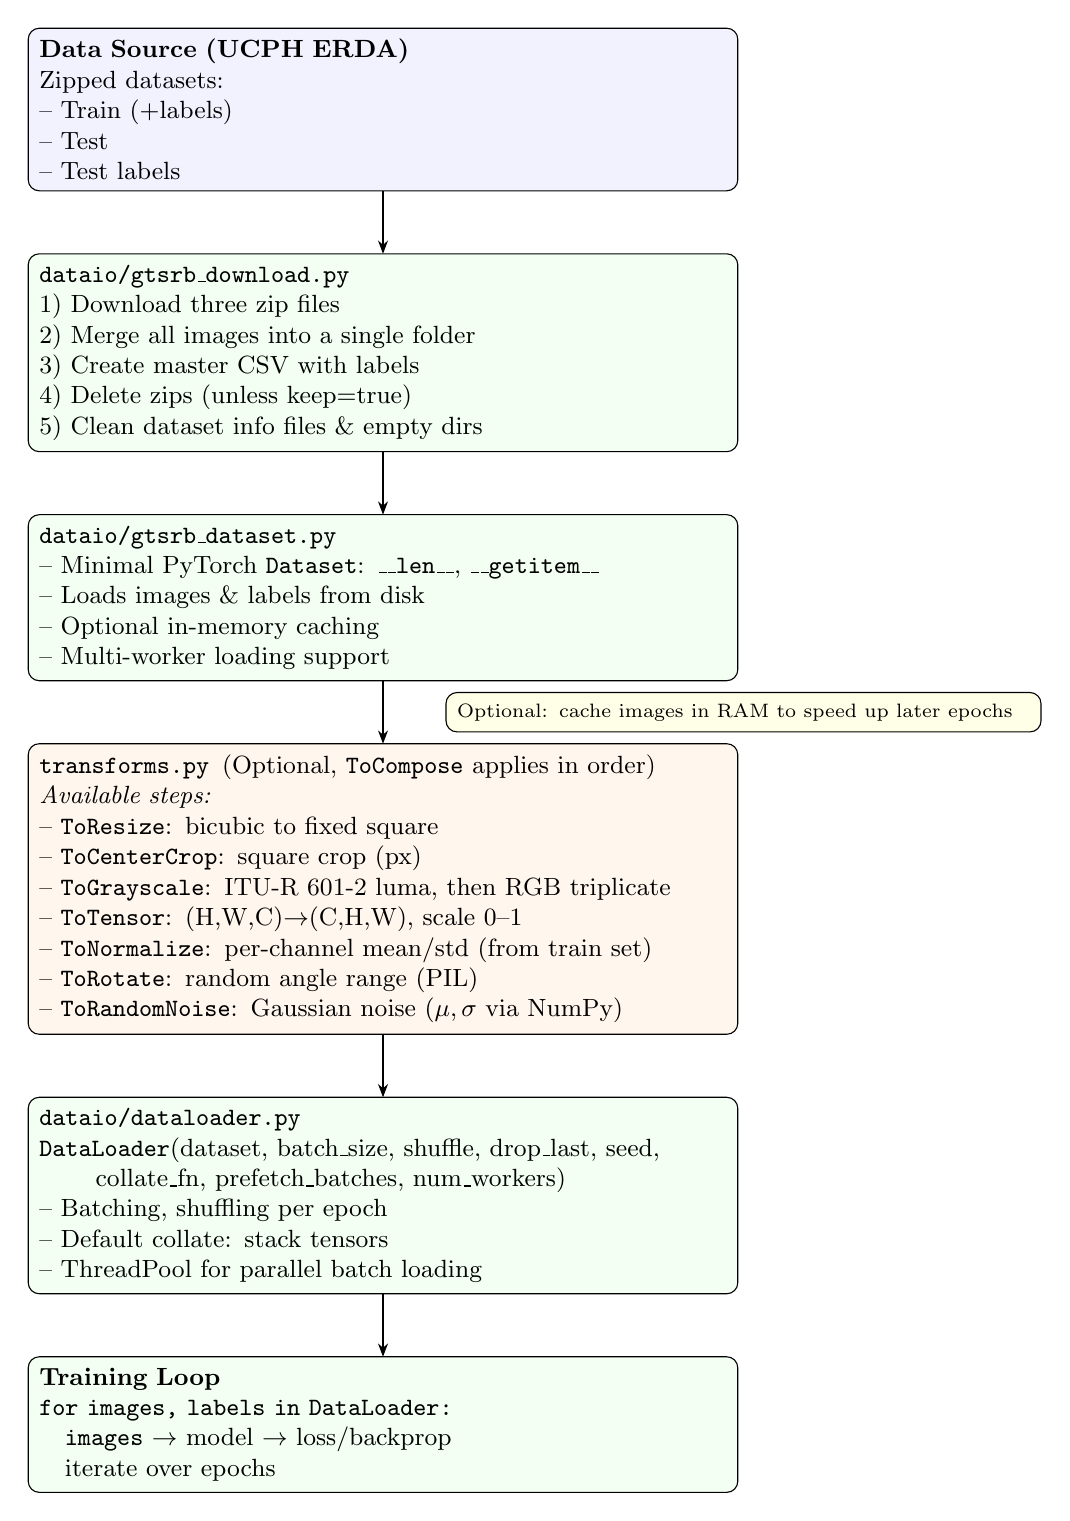
\begin{tikzpicture}[
        node distance=8mm,
        >=Stealth,
        font=\small,
        box/.style={draw, rounded corners, align=left, inner sep=4pt, outer sep=0pt, fill=gray!5},
        io/.style={box, fill=blue!5},
        proc/.style={box, fill=green!5},
        group/.style={box, fill=orange!7},
        note/.style={box, fill=yellow!10, font=\scriptsize},
        every node/.append style={text width=0.72\linewidth}
      ]

      % --- Nodes (stacked vertically to stay narrow) ---
      \node[io] (src) {\textbf{Data Source (UCPH ERDA)}
        \\Zipped datasets:
        \\-- Train (+labels)
        \\-- Test
        \\-- Test labels};

      \node[proc, below=of src] (dl) {\textbf{\texttt{dataio/gtsrb\_download.py}}
      \\1) Download three zip files
      \\2) Merge all images into a single folder
      \\3) Create master CSV with labels
      \\4) Delete zips (unless keep=true)
      \\5) Clean dataset info files \& empty dirs};

      \node[proc, below=of dl] (ds) {\textbf{\texttt{dataio/gtsrb\_dataset.py}}
        \\-- Minimal PyTorch \texttt{Dataset}: \texttt{\_\_len\_\_}, \texttt{\_\_getitem\_\_}
        \\-- Loads images \& labels from disk
        \\-- Optional in-memory caching
        \\-- Multi-worker loading support};

      % Transforms group
      \node[group, below=of ds] (tf) {\textbf{\texttt{transforms.py}} \,(Optional, \texttt{ToCompose} applies in order)
        \\\textit{Available steps:}
        \\-- \texttt{ToResize}: bicubic to fixed square
        \\-- \texttt{ToCenterCrop}: square crop (px)
        \\-- \texttt{ToGrayscale}: ITU-R 601-2 luma, then RGB triplicate
        \\-- \texttt{ToTensor}: (H,W,C)$\to$(C,H,W), scale 0--1
        \\-- \texttt{ToNormalize}: per-channel mean/std (from train set)
        \\-- \texttt{ToRotate}: random angle range (PIL)
        \\-- \texttt{ToRandomNoise}: Gaussian noise (\(\mu,\sigma\) via NumPy)};

      \node[proc, below=of tf] (dlr) {\textbf{\texttt{dataio/dataloader.py}}
        \\\texttt{DataLoader}(dataset, batch\_size, shuffle, drop\_last, seed,
        \\\hspace*{2.2em}collate\_fn, prefetch\_batches, num\_workers)
        \\-- Batching, shuffling per epoch
        \\-- Default collate: stack tensors
        \\-- ThreadPool for parallel batch loading};

      \node[proc, below=of dlr] (train) {\textbf{Training Loop}
        \\\texttt{for images, labels in DataLoader:}
        \\\hspace*{1em}\texttt{images} \(\to\) model \(\to\) loss/backprop
        \\\hspace*{1em}iterate over epochs};

      % --- Arrows ---
      \draw[->] (src) -- (dl);
      \draw[->] (dl) -- (ds);
      \draw[->] (ds) -- node[right, note, xshift=8mm, text width=0.6\linewidth]
      {Optional: cache images in RAM to speed up later epochs} (tf);
      \draw[->] (tf) -- (dlr);
      \draw[->] (dlr) -- (train);

    \end{tikzpicture}%
  }
  \caption{GTSRB data pipeline from download \(\rightarrow\) dataset \(\rightarrow\) transforms \(\rightarrow\) dataloader \(\rightarrow\) training.}
  \label{fig:pipeline}
\end{figure}


\begin{figure}[ht]
  \centering
  \resizebox{\linewidth}{!}{%
    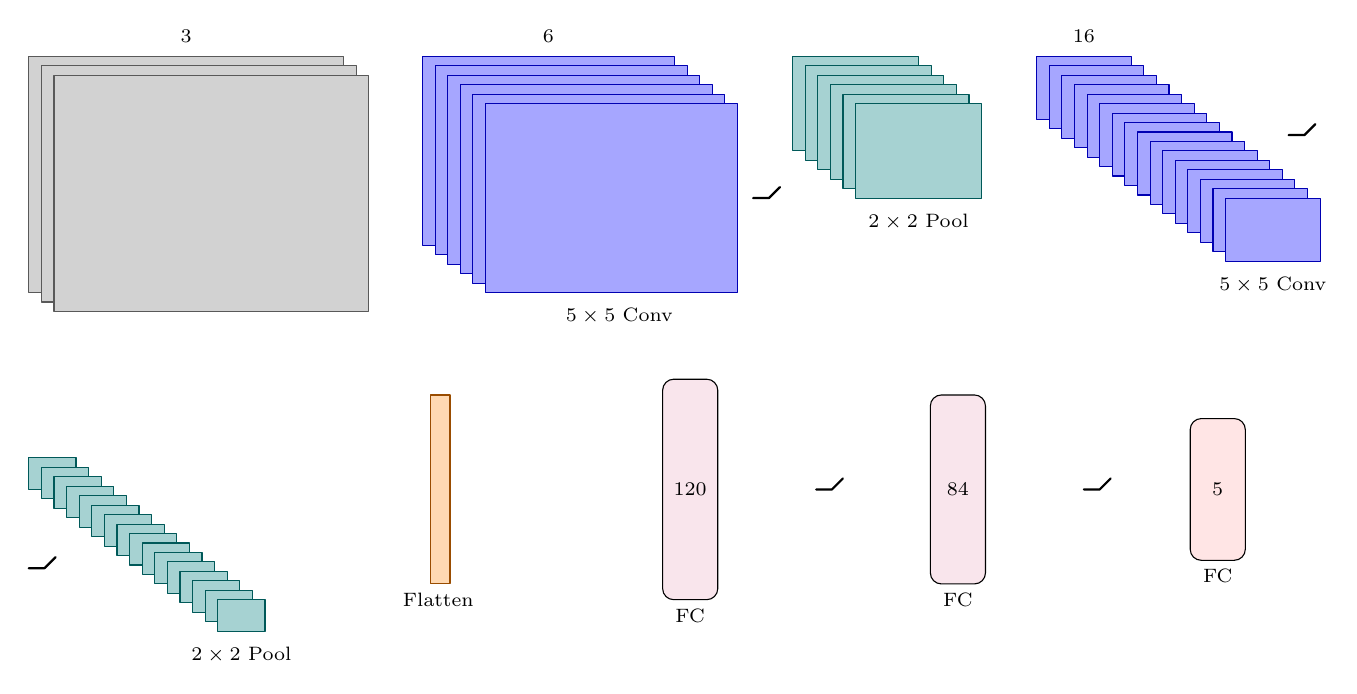
\begin{tikzpicture}[
        >=Stealth, line join=round, line cap=round,
        font=\scriptsize, x=1cm, y=1cm,
        fcbox/.style={draw, rounded corners, minimum width=7mm, minimum height=28mm, fill=purple!10},
        lbl/.style={font=\scriptsize, inner sep=1pt}
      ]
      % ---- helpers ----
      \def\dx{0.16}   % layer stack x-offset
      \def\dy{0.12}   % layer stack y-offset
      \newcommand{\maps}[6]{% x, y, w, h, color, lastIndex
        \begin{scope}[shift={(#1,#2)}]
          \foreach \i in {0,...,#6} {
              \draw[draw=#5!70!black, fill=#5!35] (\i*\dx,-\i*\dy) rectangle ++(#3,#4);
            }
        \end{scope}
      }

      %==================== ROW 1: first four steps ====================
      \def\yA{0} % y for first row

      % 1) Input (3)
      \maps{0}{\yA}{4.0}{3.0}{gray}{2}
      \node[lbl] at (2,\yA+3.25) {$3$};

      % 2) Conv5x5 → 6
      \maps{5}{\yA+0.6}{3.2}{2.4}{blue}{5}
      \node[lbl] at (6.6,\yA+3.25) {$6$};

      % 3) MaxPool2x2
      \maps{9.7}{\yA+1.8}{1.6}{1.2}{teal}{5}

      % 4) Conv5x5 → 16
      \maps{12.8}{\yA+2.2}{1.2}{0.8}{blue}{15}
      \node[lbl] at (13.4,\yA+3.25) {$16$};


      %==================== ROW 2: last five steps =====================
      \def\yB{-2.5} % y for second row (spaced below)
      \def\xStart{0} % left start for second row

      % 5) MaxPool2x2
      \maps{\xStart}{\yB}{0.6}{0.4}{teal}{15}

      % 6) Flatten (thin slab)
      \draw[fill=orange!30, draw=orange!60!black] (\xStart+5.1,\yB-1.2) rectangle ++(0.25,2.4);

      % 7) FC 120
      \node[fcbox] (fc1) at (\xStart+8.4,\yB) {$120$};
      % 8) FC 84
      \node[fcbox, minimum height=24mm] (fc2) at (\xStart+11.8,\yB) {$84$};
      % 9) FC 5 (logits)
      \node[fcbox, minimum height=18mm, fill=red!10] (fc3) at (\xStart+15.1,\yB) {$5$};


      % small ReLU markers (triangles) after convs and FCs
      \foreach \x/\y in {
          9.2/\yA+1.2,
          16/\yA+2,
          \xStart/\yB-1,
          \xStart+10/\yB,
          \xStart+13.4/\yB
        } {
          \draw[black, thick] (\x,\y) -- ++(0.2,0) -- ++(0.14,0.14);
        }

      % labels for minimal cues (kept tiny)
      \node[lbl] at (7.5,\yA-0.3) {$5 \times 5$ Conv};
      \node[lbl] at (11.3,\yA+0.9) {$2 \times 2$ Pool};
      \node[lbl] at (15.8,\yA+0.1) {$5 \times 5$ Conv};
      \node[lbl] at (\xStart+2.7,\yB-2.1) {$2 \times 2$ Pool};
      \node[lbl] at (\xStart+5.2,\yB-1.4) {Flatten};
      \node[lbl] at (\xStart+8.4,\yB-1.6) {FC};
      \node[lbl] at (\xStart+11.8,\yB-1.4) {FC};
      \node[lbl] at (\xStart+15.1,\yB-1.1) {FC};

    \end{tikzpicture}%
  }
  \caption{Visual representation of our model architecture. The presence of a small ReLU marker indicates a ReLU activation after that layer.}
\end{figure}



\end{document}
